 We extend the following example in~\cite{MMS08} with probability, to show how a probabilistic system is modeled.
 \begin{example}\label{ssec:ex}
Suppose there are $m$ jobs $\{J_1, \cdots, J_m\}$, and $q$ tasks $\{T_0, \cdots, T_n\}$. Each job is consisted of a set of tasks.
A system, consisting of $n$ workers, specifies a sequence of tasks for each worker. A task sequence for player $i$ is denoted as $\mathcal{T}_i=\langle \tau(i,0), \cdots, \tau(i, l_i)\rangle$, where $l_{i}+1$ is the length of the sequence. When finishing one task, a work waits for the rewards. Once the rewards are received, the worker starts the next task. After finishing all tasks in the sequence (i.e., after finishing $\tau(i, l)$), a worker repeats the sequence of tasks from beginning (i.e., task $\tau(i,0)$). Once a job is completed, the rewards are granted to the works who finished the tasks that compose the job. Assume that tasks for different jobs do not overlap. In completing a job, if more than one workers finish the same task, all of them will be rewarded.
A worker may deviate from the system by delaying execution of a task or not executing a task in his task sequence.

We extend the above example system with probability. In addition to the task sequence, each worker is assigned a probability $0.4$ to take the next task, and probability $0.6$ to skip the next task. For example, a work will toss a coin before taking the next task: if it is head, he takes the next task, if it is tail, he skip the next task.
\end{example}

Similar to the formalization in~\cite{MMS08}, in the example, a worker's states are modelled as $X_i=Y_i\times Z_i$, where $Y_i$ is the worker's task sequence and $Z_i$ is the status of each task, $Z_i=\{0, 1, 2\}$, with $0$ denoting that the worker is not working, $1$ denoting that the work finishes his assigned work, and $2$ denoting that the current (finished) work is used by a job. Note that in this example, the states for altruistic, rational or Byzantine players/workers are exactly the same.
%
A player's initial state is $I_i=(\tau(i,0),0)$. Since the only deviation is not taking the task, the set of actions for all players are the same, i.e., $A_i=\{a^i_0, a^i_1\}$, where $a^i_0$
denotes the player $i$ does not take the task, and $a^i_1$ denotes that the player $i$ will take the task. The action $a_1$ will lead a state $(\tau(i, j), 0)$ to $(\tau(i, j), 1)$, and the action $a_0$ leads to a self-loop. The transition from $(\tau(i, j), 1)$ to $(\tau(i, j), 2)$ happens if the task $\tau(i, j)$ is used for a job. Note that it does not needs actions from players.
Hence, $S=\langle (Y_1, Z_1), \cdots, (Y_n, Z_n)\rangle$, $I=\langle(\tau(1,0), 0),\cdots,(\tau(n,0),0)\rangle$ and $A=\{\{a^1_0, a^1_1\}, \cdots, \{a^n_0, a^n_1\}\}$.

We use the function $\pi_i$ to project a global state $s$ or a global action $a$ to the local state of player $i$, and use $a^i_{\tau}$ to denote the empty action of player $i$. The function $B_i(s, a, s')$ is defined as follows:
\[
\begin{array}{l}
B_i(s, a_i, s')=\\
\ \left\{
\begin{array}{ll}
\mbox{true} &\mbox{if}\ \pi_i(s)=(\tau(i,j),0), \pi_i(s')=(\tau(i,j), 0), a_i=a^i_0\\
\mbox{true} & \mbox{if}\ \pi_i(s)=(\tau(i,j),0), \pi_i(s')=(\tau(i,j), 1),a_i=a^i_1\\
%\mbox{true} & \mbox{if}\ \pi_i(s)=(\tau(i,j),1), \pi_i(s')=(\tau(i,j), 2), a_i=a^i_{\tau}\\
%            & \tau(i,j)\ \mbox{is completed and needed for a job}\\
%\mbox{true} & \mbox{if}\ \pi_i(s)=(\tau(i,j),1), \pi_i(s')=(\tau(i,j), 1), a_i=a^i_{\tau}\\
%            &\tau(i,j)\ \mbox{is not completed or not needed for a job}\\
%\mbox{true} & \mbox{if}\ \pi_i(s)=(\tau(i,j),2), \pi_i(s')=(\tau(i,(j+1)\%l_i), 0), a_i=a^i_{\tau}\\
\mbox{false}& \mbox{otherwise}
\end{array}
\right.
\end{array}
\]
The first case says that if a player $i$'s next job is $j$, he can choose to not take the task ($a_i=a^i_0$), and this action leads to a state where $i$'s local state does not change ($\pi_i(s')=\pi_i(s)$). The second case models that if the player takes the task ($a_i=a^i_1$), the action leads to a state where the local state of $i$ changes into $\tau(i,j), 1)$.
%The third case represents that if the player's task is finished and is used for a job, then the status of his task is changed to $2$, otherwise, the status of the task remains to be $1$ (the fourth case). The fifth case states that if the task is rewarded, then the system automatically transit the state of the player to the beginning status of the next task. 

Differing from the definition in~\cite{MMS08}, the function $T_i(s,a_i)$ in this system is defined exactly the same as $B_i(s,a_i)$, since both of the actions $a^i_0$ and $a^i_1$ are enabled in the probabilistic system.
\begin{equation*}
T_i(s,a_i)=
\begin{cases}
\mbox{true} &\mbox{if}\ \pi_i(s)=(\tau(i,j),0), a_i=a^i_0\\
\mbox{true} & \mbox{if}\ \pi_i(s)=(\tau(i,j),0), a_i=a^i_1\\
\mbox{false} & \mbox{otherwise} 
\end{cases}
\end{equation*}
%\begin{figure}
%	\centering
%	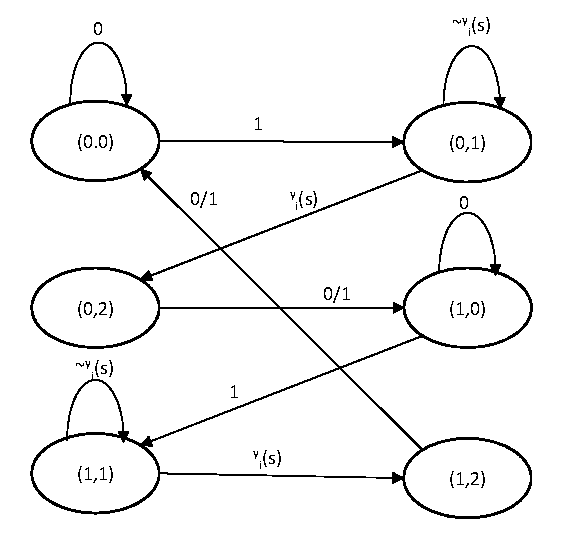
\includegraphics[width=\columnwidth]{state_diagram_cropped}
%	\caption{State Diagram Example}
%	\label{fig:state_diagram_ex}
%\end{figure}
%For instance, assume there are $3$ workers, worker $W_1$, assigned job $J_1$, worker $W_2$ assigned job $J_2$, and %worker $W_3$ assigned job $J_1$. The task sequence of $W_1$ is $T_0,T_1,T_0,T_1,T_0,T_1 \cdots$, the task sequence of %$W_2$ is $T_1,T_0,T_1,T_0,T_1\cdots$. For each task, a worker has $3$ states, denoted by the value of $Z_i$: $z_i=0$ %means that the worker does not start working on the task; $z_i=1$ means that the worker is working on the task; and $z_i=2$ %means that the worker has completed the task. Let $Y_i= \{0,1\}$ where $0$ and $1$ denoting the position index in $\tau_i$. %State space for worker $i$ is $Y_i \times Z_i$. Let the initial local state of all the workers be $I=(0,0)$.

%The function $\gamma _i(s)$ denotes whether the current task is already completed at the global state $s$. This is sufficient to %show the involvement of the global state in the automata $B_i$. The function defines set of global states that are allowed to %arrive at the completed state at the presence of any input. ($a_i = 1$ or $a_i = 0$). The knowledge about global state is %considered to be transparent. Evaluation of the function will be discussed later. Now, we can define the pay-off function $h_i$.
The payoff function is defined the same as original as follows.
\begin{equation*}
\text{$h^{\psi}_i(s_i,a_i)=$}
\begin{cases}
\text{-1} &  \text{$\pi_i(s)=(\tau(i,j),0) \wedge (a_i = a^i_1) $} \\
\text{4} & \text{$\pi_i(s)=(\tau(i,j),2)$} \\
\text{0} & \text{otherwise}
\end{cases}	
\end{equation*}
The first case represents that the player works for a task, meaning that the player is paying, instead of gaining, and thus the payoff is negative. 
The second case capture the situation that the player's task is used in a job and thus the player is paid with positive payoff value. If the player does not work then he gains nothing and pays nothing, and thus has payoff value $0$. 

The probabilistic function $P_i(s, a_i)$ is defined for altruistic player as follows:
\begin{equation*}
P_i(s_i, a_i)=
\begin{cases}
%\left\{
%\begin{array}{ll}
%p& \mbox{if}\ i\in Z, a_i=a^i_0\\
%1-p &\mbox{if}\ i\in Z, a_i=a^i_1\\
%&\mbox{where}\ p\ \mbox{is any value between}\ 0\ \mbox{and}\ 1\\
%\end{array}
%\right.\\

\begin{array}{ll}
0.6& \mbox{if}\  a_i=a^i_0\\
0.4 &\mbox{if}\  a_i=a^i_1
\end{array}

\end{cases}
\end{equation*}
If a player is a Byzantine player $i\in Z$, then the probability can be an arbitrary distribution ($p$ can be any value between and include $0$ and $1$).
If a player is an altruistic player $i\not\in Z$, the probability distribution is pre-defined by the system ($0.6$ for not taking the task and $0.4$ for taking the task).

%Finally, all actions of a player are probabilistic, hence, $PA_i(s)$ is defined as follows:
%\begin{equation*}
%PA_i(s)=
%\begin{cases}
%\{a^i_0, a^i_1\} & \mbox{if}\ T_i(s,a_i)=\mbox{true}\\
%\emptyset & \mbox{otherwise}
%\end{cases}
%\end{equation*}
%$z_i=2$ only if a job is completed. In this case all the workers who took part to complete the tasks corresponding to the job %receive, a pay-off of $4$. First case corresponds to working on a non completed task where the worker receives a pay-off of %$-1$. Second case denotes the scenario of completing a job and in that situation, all the workers involved in the tasks %corresponding to the job, receive a utility of $4$ each.  $T_i$ in this mechanism is the same state machine without the %transitions corresponding to ($a_i = 0$).

%This mechanism can be easily extended to a probabilistic version by introducing $P(s,a)$. \newline
%$P(s,1)=0.4$ , $P(s,0)=0.6$.
